\documentclass{article}
\usepackage[utf8]{inputenc}

\title{Filtro di Kalman}
\author{Antonio Lanciotti, Lorenzo D'Agostino, Arment Pelivani}
\date{March 2019}

\usepackage{natbib}
\usepackage{graphicx}
\usepackage{caption}
\captionsetup[figure]{labelformat=empty}
\begin{document}

\maketitle

\begin{figure}[ht]
\centering
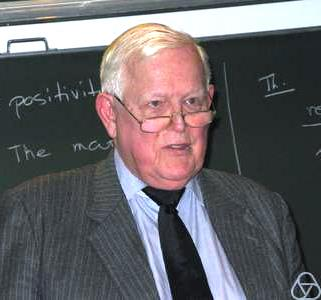
\includegraphics[scale=1]{Rudolf_Kalman.jpg}
\caption{Rudolf E. Kalman}
\label{fig:kalman}
\end{figure}

\section{Introduzione}
Il filtro di Kalman è un osservatore asintotico dello stato per sistemi lineari tempo-invarianti in presenza di rumori gaussiani.

\newpage

\section{Conclusione}
``A nonlinear differential equation of the Riccati type is derived for the covariance matrix of the optimal filtering error. The solution of this 'variance equation' completely specifies the optimal filter for either finite or infinite smoothing intervals and stationary or non-stationary statistics.
The variance equation is closely related to the Hamiltonian (canonical) differential equations of the calculus of variations. Analytic solutions are available in some cases. The significance of the variance equation is illustrated by examples which duplicate, simplify, or extend earlier results in this field.
The duality principle relating stochastic estimation and deterministic control problems plays an important role in the proof of theoretical results. In several examples, the estimation problem and its dual are discussed side-by-side.
Properties of the variance equation are of great interest in the theory of adaptive systems. Some aspects of this are considered briefly. '' \citep{kalmanbucy}

\bibliographystyle{plain}
\bibliography{references}
\end{document}
